\subsection{SGX Security Properties}
\label{sec:sgx_security_analysis}

We have summarized SGX's programming model and the implementation details
that are publicly documented in Intel's official documentation and published
patents. We are now ready to bring this the information together in an analysis
of SGX's security properties. We start the analysis by re-starting SGX's
security guarantees, and spend the bulk of this section discussing how SGX
fares when pitted against the attacks described in
\S~\ref{sec:security_background}.


\subsubsection{Overview}

Intel's Software Guard Extensions (SGX) is Intel's latest iteration of a
trusted hardware solution to the secure remote computation problem. The SGX
design is centered around the ability to create an isolated container whose
contents receives special hardware protections that are intended to translate
into privacy, integrity, and freshness guarantees.

% ISCA 2015 SGX: Slide 93

An enclave's initial contents is loaded by the system software on the computer,
and therefore cannot contain secrets in plain text. Once initialized, an
enclave is expected to participate in a software attestation process, where it
authenticates itself to a remote server. Upon successful authentication, the
remote server is expected to disclose some secrets to an enclave over a
secure communication channel. The SGX design attempts to guarantee that the
measurement presented during software attestation accurately represents the
contents loaded into the enclave.

SGX also offers a certificate-based identity system that can be used to migrate
secrets between enclaves that have certificates issued by the same authority.
The migration process involves securing the secrets via authenticated
encryption before handing them off to the untrusted system software, which
passes them to another enclave that can decrypt them.

The same mechanism used for secret migration can also be used to cache the
secrets obtained via software attestation in an untrusted storage medium
managed by system software. This caching can reduce the number of times that
the software attestation process needs to be performed in a distributed system.
In fact, SGX's software attestation process is implemented by enclaves with
special privileges that use the certificate-based identity system to securely
store the CPU's attestation key in untrusted memory.


\subsubsection{Physical Attacks}
\label{sec:sgx_vs_physical_attacks}

We beging by discussing SGX's resilience to the physical attacks described in
\S~\ref{sec:physical_attacks}. Unfortunately, this section is set to disappoint
readers expecting definitive statements. The lack of publicly available details
around the hardware implementation aspects of SGX precludes any rigurous
analysis. However, we do know enough about SGX's implementation to point out a
few avenues for future exploration.

Due to insufficient documentation, one can only hope that the SGX security
model is not trivially circumvented by a port
attack~(\S~\ref{sec:physical_port_attacks}). We are particularly concerned
about the Generic Debug eXternal
Connection~(GDXC)~\cite{yuffe2011sandybridge, intel2011gdxc}, which collects
and filters the data transfered by the uncore's ring bus
(\S~\ref{sec:cache_coherence}), and reports it to an external debugger.

The SGX memory protection measures are implemented at the core level, in the
PMH (\S~\ref{sec:sgx_access_protection}) and at the chip die level, in the
memory controller (\S~\ref{sec:sgx_uncore_modifications}). Therefore, the code
and data inside enclaves is stored in plaintext in on-chip
caches~(\S~\ref{sec:caching}), which entails that the enclave contents travels
without any cryptographic protection on the uncore's ring bus
(\S~\ref{sec:cache_coherence}).

Fortunately, a recent Intel patent~\cite{shanbhogue2015gdxcsgx} indicates that
Intel engineers are tackling at least some classes of attacks targeting
debugging ports.

The SDM and SGX papers discuss the most obvious class of bus tapping
attacks~(\S~\ref{sec:physical_bus_attacks}), which is the DRAM bus tapping
attack. SGX's threat model considers DRAM and the bus connecting it to the CPU
chip to be untrusted. Therefore, SGX's Memory Encryption
Engine~(MEE,~\S~\ref{sec:sgx_uncore_modifications}) provides privacy, integrity
and freshness guarantees to the Enclave Page Cache~(EPC,~\S~\ref{sec:sgx_epc})
data while it is stored in DRAM.

However, both the SGX papers and the ISCA 2015 tutorial on SGX admit that the
MEE does not protect the addresses of the DRAM locations accessed when cache
lines holding EPC data are evicted or loaded. This provides an opportunity for
a malicious computer owner to observe an enclave's memory access patterns by
combining a DRAM address line bus tap with carefully crafted system software
that creates artifical pressure on the last-level
cache~(LLC~,\S~\ref{sec:caching}) lines that hold the enclave's EPC pages.

On a brighter note, as mentioned in \S~\ref{sec:physical_bus_attacks}, we are
not aware of any successful DRAM address line bus tapping attack. Furthermore,
SGX is vulnerable to cache timing attacks that can be carried out completely in
software, so malicious computer owners do not need to bother setting up a
physical attack to obtain an enclave's memory access patterns.

While the SGX documentation addresses DRAM bus tapping attacks, it makes no
mention of the System Management bus~(SMBus,~\S~\ref{sec:intel_me}) that
connects the Intel Management Engine~(ME,~\S~\ref{sec:intel_me}) to various
components on the computer's motherboard.

In \S~\ref{sec:sgx_vs_device_attacks}, we will explain that the ME might play a
role in SGX's software attestation process. This makes us concerned about the
possibility of an attack that taps the SMBus to reach into the Intel ME. The
SMBus is much more accessible than the DRAM bus, as it has fewer wires that
operate at a significantly lower speed. Unfortunately, without more information
about the role that the Intel ME plays in a computer, we cannot move beyond
speculation on this topic.

The threat model stated by the SGX design excludes physical attacks targeting
the CPU chip~(\S~\ref{sec:physical_chip_attacks}). Fortunately, Intel's patents
disclose an array of countermeasures aimed at increasing the cost of chip
attacks.

For example, the original SGX patents~\cite{intel2013patent1, intel2013patent2}
disclose that the Fused Seal Key and the Provisioning Key, which are stored in
e-fuses (\S~\ref{sec:sgx_quoting_enclave}), are encrypted with a \textit{global
wrapping logic key}~(GWK). The GWK is a 128-bit AES key that is hard-coded in
the processor's circuitry, and serves to increase the cost of extracting the
keys from an SGX-enabled processor.

As explained in \S~\ref{sec:physical_chip_attacks}, e-fuses have a large
feature size, which makes them relatively easy to ``read'' using a
high-resolution microscope. In comparison, the circuitry on the latest Intel
processors has a significantly smaller feature size, and is more difficult to
reverse engineer. Unfortunately, the GWK is shared among all the chip dies
created from the same mask, so it has all the drawbacks of global secrets
explaiend in \S~\ref{sec:physical_chip_attacks}.

Newer Intel patents~\cite{gotze2014provisioning, gotze2014provisioning2}
disclose that SGX-enabled processors also employ a
\textit{Physically Unclonable Function}~(PUF,~\cite{suh2007puf}), which
generates a symmetric key that is used during the provisioning process.

Specifically, at an early provisioning stage, the PUF key is encrypted with the
GWK and transmitted to the key generation server. At a later stage, the key
generation server encrypts the key material that will be burned into the
processor chip's e-fuses with the PUF key, and transmits the encrypted material
to the chip. The PUF key increases the cost of obtaining a chip's fuse key
material, as an attacker must compromise both provisioning stages in order to
be able to decrypt the fuse key material.

As mentioned in previous sections, patents reveal design possibilities
considered by the SGX engineers. However, due to the length timelines involved
in patent applications, patents necessarily describe earlier versions of the
SGX implementation plans, which might not match the shipping implementation. We
expect this might be the case with the PUF provisioning patents, as it makes
little sense to include a PUF in a chip die and rely on e-fuses and a GWK to
store SGX's root keys. Deriving the root keys from the PUF would be more
resilient to chip imaging attacks.

SGX's threat model excludes power analysis
attacks~(\S~\ref{sec:power_analysis_attacks}) and other side-channel attacks.
This is understandable, as power attacks cannot be addressed at the
architectural level. Defending against power attacks requires expensive
countermeasures at the lowest levels of hardware implementation, which can only
be designed by engineers who have deep expertise in both system security and
Intel's manufacturing process. It follows that defending against power analysis
attacks has a very high cost-to-benefit ratio.


\subsubsection{Memory Mapping Attacks}
\label{sec:sgx_vs_memory_mapping_attacks}

\S~\ref{sec:sgx_threads} explained that the code running inside an enclave uses
the same address translation process~(\S~\ref{sec:paging}) and page tables as
its host application. While this design approach makes it easy to retrofit SGX
support into existing codebases, it also enables the address translation
attacks described in \S~\ref{sec:address_translation_attacks}.

The SGX design protects the code inside enclaves against the active attacks
described in \S~\ref{sec:address_translation_attacks}. These protections have
been extensively discussed in prior sections, so we limit ourselves to
pointing out SGX's answer to each active attack. We also explain the lack of
protections against passive attacks, which can be used to learn an enclave's
memory access pattern at 4KB page granularity.

SGX uses the Enclave Page Cache Map~(EPCM,~\S~\ref{sec:sgx_epcm}) to store each
EPC page's position in its enclave's virtual address space. The EPCM is
consulted by SGX's extensions to the Page Miss
Handler~(PMH,~\S~\ref{sec:sgx_access_concepts}), which prevent straightforward
active address translation attacks~(\S~\ref{sec:memory_mapping_attacks}) by
rejecting undesirable address translations before they reach the
TLB~(\S~\ref{sec:tlbs}).

SGX allows system software to evict~(\S~\ref{sec:sgx_epc_eviction}) EPC pages
into untrusted DRAM, so that the EPC can be over-subscribed. The contents of
the evicted pages and the associated EPCM metadata are protected by
cryptographic primitives that offer privacy, integrity and freshness
guarantees. This protects against the active attacks using page swapping
described in \S~\ref{sec:page_swapping_attacks}.

When system software wishes to evict EPC pages, it must follow the process
described in \S~\ref{sec:sgx_eblock}, which guarantees to the SGX
implementation that all the logical processors~(LPs,~\S~\ref{sec:cpu_core})
have invalidated any TLB entry associated with pages that will be evicted. This
defeats the active attacks based on stale TLB entries described in
\S~\ref{sec:tlb_mapping_attacks}.

\S~\ref{sec:sgx_access_correctness} outlines a correctness proof for all the
protection measures described above.

Unfortunately, SGX does not protect against passive address translation
attacks~(\S~\ref{sec:fault_tracking_attacks}), which can be used to learn an
enclave's memory access pattern at page granularity. While this appears
beningn, recent work \cite{xu2015pagefaults} demonstrates the use of these
passive attacks in a few practical settings, which are immediately concerning
for image processing applications.

The rest of this section describes the theory behind planning a passive attack
against an SGX enclave. The reader is directed to \cite{xu2015pagefaults} for
a fully working system.

Passive address translation attacks rely on the fact that memory accesses
issued by SGX enclaves go through the Intel architecture's address translation
process~(\S~\ref{sec:paging}), including delivering page
faults~(\S~\ref{sec:faults}) and setting the accessed (A) and dirty (D)
attributes~(\S~\ref{sec:page_table_attributes}) on page table entries.

A malicious OS kernel or hypervisor can obtain the page-level trace of an
application executing inside an enclave by setting the present (P) attribute to
0 on all the enclave's pages before starting enclave execution. While an
enclave executes, the malicious system software maintains exactly one
instruction page and one data page present in the enclave's address space.

When a page fault is generated, CR2 contains the virtual address of a page
accessed by enclave, and the error code indicates whether the memory access was
a read or a write (bit 1) and whether the memory access is a data access or
an instruction fetch access (bit 4). On a data access, the kernel tracing the
enclave code's memory access pattern would set the P flag of the desired page
to 1, and set the P flag of the previously accessed data page to 0. Instruction
accesses can be handled in a similar manner.

For a slightly more detailed trace, the kernel can set a desired page's
writable (W) attribute to 0 if the page fault's error code indicates a read
access, and only set it to 1 for write accesses. Also, applications that use a
page as both code and data (self-modifying code and just-in-time compiling VMs)
can be handled by setting a page's disable execution (XD) flag to 0 for a data
access, and by carefully accounting for the case where the last accessed data
page is the same as the last accessed code page.

Leaving an enclave via an Asynchronous Enclave Exit~(AEX,~\S~\ref{sec:sgx_aex})
and re-entering the enclave via \texttt{ERESUME}~(\S~\ref{sec:sgx_eresume})
causes the CPU to flush TLB entries that contain enclave addresses, so a
tracing kernel would not need to worry about flushing the TLB. The tracing
kernel does not need to flush the caches either, because the CPU needs to
perform address translation even for cached data.

A straightforward way to reduce this attack's power is to increase the page
size, so the trace contains less information. However, the attack cannot be
completely prevented without removing the kernel's ability to oversubscribe the
EPC, which is a major benefit of paging.


\subsubsection{Software Attacks on Peripherals}
\label{sec:sgx_vs_device_attacks}

The SGX threat model considers system software to be untrusted, which is
necessary for SGX to qualify as a solution to the security issues encountered
in Infrastructure-as-a-Service (IaaS) cloud computing deployments. Since the
SGX design does not trust the system software, it must be prepared to withstand
the attacks described in \S~\ref{sec:device_attacks}, which can be carried out
by the system software thanks to its ability to control peripheral devices on
the computer's motherboard~(\S~\ref{sec:motherboard}). This section summarizes
the security properties of SGX when faced with these attacks, based on publicly
available information.

When SGX is enabled on an LP, it configures the memory
controller~(MC,~\S~\ref{sec:cache_coherence}) integrated on the CPU chip die to
reject any DMA transfer that falls within the Processor Reserved
Memory~(PRM,~\S~\ref{sec:sgx_prm}) range. The PRM includes the EPC, so the
enclaves' contents is protected from the PCI Express attacks described in
\S~\ref{sec:pcie_attacks}. This protection guarantee relies on the fact that
the MC is integrated on the processor's chip die, so the MC configuration
commands issued by SGX's microcode
implementation~(\S~\ref{sec:sgx_microcode_modifications}) are transmitted over
a communication path that never leaves the CPU die, and therefore can be
trusted.

SGX regards DRAM as an untrusted storage medium, and uses cryptographic
primitives implemented in the MEE to guarantee the privacy, integrity and
freshness of the EPC contents that is stored into DRAM. This protects against
software attacks on DRAM's integrity, like the rowhammer attack described in
\S~\ref{sec:rowhammer_attack}.

% Interaction with Performance Monitoring: SDM S 43.6

The SDM describes an array of measures that SGX takes to disable processor
features intended for debugging when a LP starts executing an enclave's code.
For example, enclave entry~(\S~\ref{sec:sgx_eenter}) disables Precise Event
Based Sampling (PEBS) for the LP, as well as any hardware breakpoints placed
inside the enclave's virtual address range~(ELRANGE,~\S~\ref{sec:sgx_elrange}).
This addresses some of the attacks described in \S~\ref{sec:perfmon_attacks},
which take advantage of performance monitoring features to get information that
typically requires access to hardware probes.

% ISCA 2015 SGX Slide 115:
%   "Software Side-Channel Adversary"

At the same time, the SDM does not mention anything about uncore PEBS counters,
which can be used to learn about an enclave's LLC activity. Furthermore, the
ISCA 2015 tutorial slides mention that \textbf{SGX does not protect against
software side-channel attacks} that rely on performance counters.

This limitation in SGX's threat model leaves security-conscious enclave authors
in a rather terrible situation. These authors know that SGX does not protect
their enclaves against a class of software attacks. At the same time, they
cannot even contemplate attempting to defeat these attacks on their own, due to
lack of information. Specifically, the documentation that is publicly available
from Intel does not provide enough information to model the information leakage
due to performance counters.

For example, Intel does not document the mapping implemented in
CBoxes~(\S~\ref{sec:cache_coherence}) between physical DRAM addresses and the
LLC slices used to cache the addresses. This mapping impacts several uncore
performance counters, and the impact is strong enough to allow security
researches to reverse-engineer the mapping \cite{inci2015rsachannel,
maurice2015intelhash, yarom2015intelhash}. Therefore, it is safe to assume that
a malicious computer owner who knows the CBox mapping can use the uncore
performance counters to learn about an enclave's memory access patterns.

The SGX papers mention that SGX's threat model includes attacks that overwrite
the flash memory chip that stores the computer's boot firmware, which result in
malicious code running in System Management Mode~(SMM,~\S~\ref{sec:rings}).
However, all the official SGX documentation is silent about the implications of
an attack that compromises the firmware executed by the Intel ME.

\S~\ref{sec:firmware_attacks} states that the ME's firmware is stored in the
same flash memory as the boot firmware, and explains that the ME has a very
broad

% Key Structures and Provisioning: Ruan 2014 Ch 5

\cite{ruan2014intelme}

This firmware
is stored in


Attacks on the Boot Firmware and Intel ME~()

\cite{costan2011spchip}



\subsubsection{Privileged Software Attacks}
\label{sec:sgx_vs_privileged_sw_attacks}


Modern Intel CPUs feature hyper-threading, which means that each core has two
(or more) sets of register files and local APICs, presented as logical
processors running separate threads (see Figure \ref{fig:cpu_core}). The
threads share the other core resources, such as the fetch and decode units,
execution units and L1 and L2 caches. SGX does not prevent hyper-threading, so
a malicious OS kernel or hypervisor can schedule a thread executing enclave
code and a snooping thread on logical processors on same core. The snooping
thread can use the processor's high-resolution performance counter
\cite{petters1999making} to get information about the instructions and memory
access patterns of the thread executing enclave code.

A promising approach for preventing against hyper-threading leaks is to
effectively disable hyper-threading, by using \texttt{CPUID} to find out the
number of logical processors in the current core, and to require the OS to
schedule threads in the same enclave on all the logical processors. This could
be implemented by having the main thread spinlock waiting for the other threads
to start, before any protected computation is performed. However, a malicious
kernel or hypervisor can de-schedule the other threads after the main thread
performed the spinlock check, so this defense is not reliable.


\subsubsection{Cache Timing Attacks}
\label{sec:sgx_vs_cache_timing_attacks}

\S~\ref{sec:cache_timing}

The AEX process and the \texttt{ERESUME} instructions do not flush the CPU
caches. A tracing kernel can take advantage of cache timing to narrow down
the addresses in an application's memory access trace to cache line
granularity, by extending the method described above with the steps below.

The tracing kernel controls the mapping between virtual addresses and physical
addresses, so it can make sure that its own code and data use different sets
in the L2 cache from the enclave's code and data. For example, in a typical
256~KB (per-core) L2 cache organized as 512 8-way sets of 64-byte lines, the
tracing kernel could allocate lines 0-63 for the enclave's code page, lines
64-127 for the enclave's data page, and use lines 128-511 for its own pages.

Right before entering an enclave via \texttt{EENTER} or \texttt{ERESUME}, the
kernel would issue \texttt{CLFLUSH} instructions to flush the enclave's code
page and data page from the cache. The enclave could have accessed a single
code page and a single data page, so flushing the cache should be reasonably
efficient. The tracing kernel then uses 16 bogus pages (8 for the enclave's
code page, and 8 for the enclave's data page) to load all the 8 ways in the 128
cache sets allocated by enclave pages. After an AEX gives control back to the
tracing kernel, it can read the 16 bogus pages, and exploit the time difference
between an L2 cache hit and a miss to see which cache lines were evicted and
replaced by the enclave's memory accesses.


% PRMRR documented in HASP papers and both SGX manuals, completely removed from
% SDM. It still exists in Coreboot. Couldn't find other Skywell code.
The SGX manual states that the EPC (the memory used to store enclave data) can
only be set up as UC or WB. While no further explanation is provided, we assume
that the UC option was provided in order to attempt to mitigate against some
cache-timing attacks.


% Access Control Requirements: SDM S 38.3

Pages that store key SGX structures cannot be accessed directly, even by the
code executing inside their enclaves. Furthermore, the SGX instructions that
operate on SGX data structures check the EPCM type fields of their inputs
against the expected types. This type system prevents software from
intentionally or accidentally corrupting the key SGX data structures.




% ECREATE forces R, W, X to 0 in the page's EPCM. EADD also forces R/W/X to 0
% if the page type in SECINFO is PT_TCS (the only special type it can create).
%
%
% EPA doesn't read any SECINFO, and uses 0 for R, W, X.

% ERESUME can be replaced by normal EENTER, XRESTOR and accounting. Describe
% and argue against ERESUME.

Enclaves were designed to contain and protect the privacy-sensitive parts of an
application. All the code that handles private data must receive integrity
protection. Otherwise, a hostile environment could modify the code to leak
information about private data. Therefore, the SGX programming model prescribes
that code which accesses private data must be entirely contained inside an
enclave. Jumping into and out of enclave code must be performed explicitly
using the dedicated instructions \texttt{EENTER} and \texttt{EEXIT}.


\begin{figure}[hbt]
  \centering
  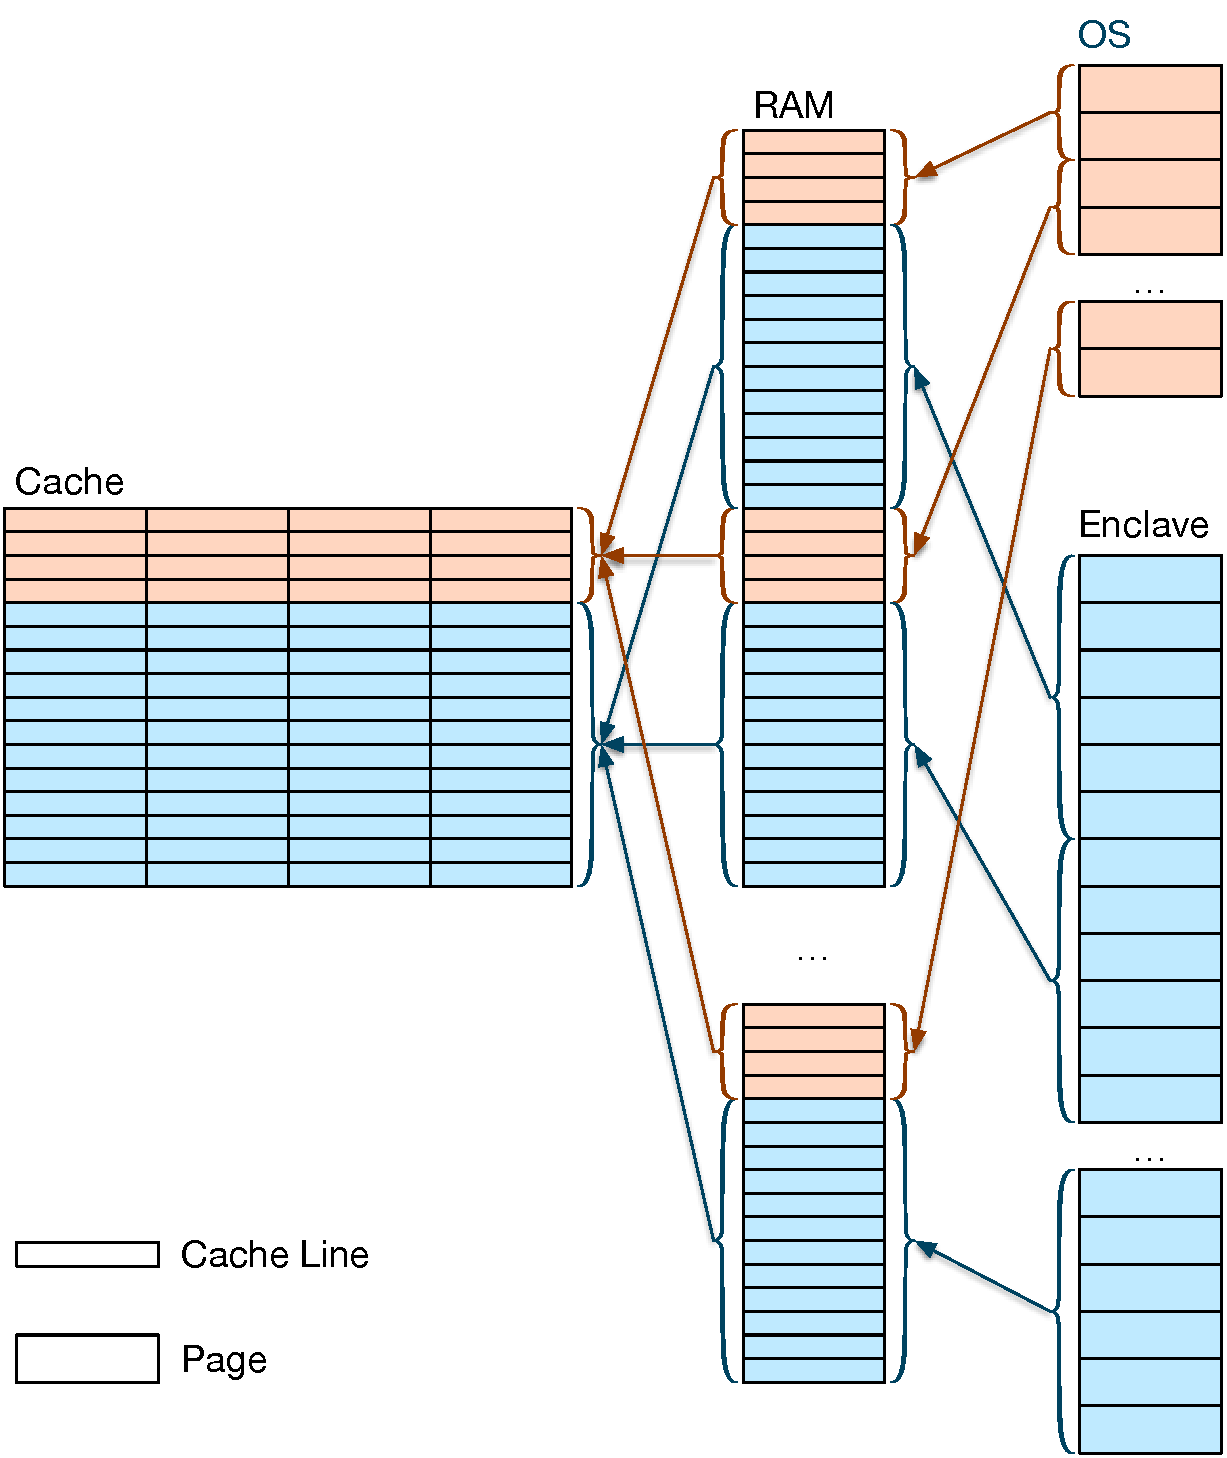
\includegraphics[width=85mm]{figures/cache_partitions.pdf}
  \caption{
    Cache partitioning between two applications. Each application has some
    cache sets allocated to it, and only uses RAM regions that map to its cache
    sets. When partitioning the L1 cache, applications have to follow this
    constraint themselves. When the L2 cache is partitioned, the OS can map the
    pages in an application's virtual address space to the RAM regions that the
    application can use, so applications are oblivious to the cache
    partitioning.
  }
  \label{fig:cache_partitions}
\end{figure}


\subsubsection{DOS Prevention}
% NOTE: This is a slightly edited answer to a question we received.

SGX enclaves execute at the lowest privilege level (user mode / ring 3), so
they cannot compromise the system software without exploiting a security
vulnerability. Therefore, the only kind of malicious behavior that an enclave
can exhibit is denial of service (DoS).

The SGX design provides system software the tools it needs to protect itself
from enclaves that engage into CPU hogging and DRAM hogging. As enclaves cannot
perform I/O directly, these are the only two classes of DoS attacks available
to them.

An enclave that attempts to hog a logical processor (CPU core on most systems)
assigned to it can be pre-empted by the system software via an Inter-Processor
Interrupt (IPI) issued from another processor. This method is available as long
as the system software reserves at least one logical processor for non-enclave
computation.

Furthermore, most OS kernels use tick schedulers, which use a real-time clock
(RTC) configured to issue periodical interrupts (ticks) to all cores. The RTC
interrupt handler invokes the kernel's scheduler, which choses the thread that
will get to use the logical processor until the next RTC interrupt is received.
Therefore, kernels that use tick schedulers always have the opportunity to
de-schedule enclave threads, and don't need to rely on the ability to send
IPIs.

In SGX, the system software can always evict an enclave's EPC pages to non-EPC
memory, and then to disk. The system software can also outright deallocate an
enclave's EPC pages, though this will probably cause the enclave code to
encounter page faults that cannot be resolved. The only catch is that the EPC
pages that hold metadata for running enclave threads cannot be evicted or
removed. However, this can easily be resolved, as the system software can
always preempt enclave threads, using one of the methods described above.

% TODO(pwnall): Move the following paragraphs into Sanctum.

Sanctum gives the system software less control over the DRAM regions allocated
to enclaves, in order to hide the enclaves' memory access patterns.
Specifically, the system software cannot reclaim a DRAM region from an enclave
without the enclave's cooperation. However, the system software can always
completely terminate an enclave and reclaim all its memory.

Sanctum's enclaves can only be terminated when all their threads are stopped.
Therefore, when the system software decides that an enclave is hogging CPU or
DRAM, it can pre-empt all the enclave's threads, using the methods described
above, and then terminate the enclave.


\subsection{Interaction with Anti-Virus Software}
% NOTE: This is a slightly edited answer to a question we received.

Today's anti-virus (AV) systems are glorified pattern matchers. AV software
simply scans all the executable files on the system and the memory of running
processes, looking for bit patterns that are thought to only occur in malicious
software. These patterns are pompously called "virus signatures".

SGX (and TXT, to some extent) provides a method for executing code in an
isolated container that we refer to as an enclave. Enclaves are isolated from
all the other software on the computer, including any AV software that might be
installed.

The isolation afforded by Sanctum (and SGX, etc.) opens up the possibility for
bad actors to structure their attacks as a generic loader that would end up
executing a malicious payload without tripping the AV's pattern matcher.  More
specifically, the attack would create an enclave and initialize it with a
generic loader that looks innocent to an AV. The loader inside the enclave
would obtain an encrypted malicious payload, and would undergo software
attestation with an Internet server to obtain the payload's encryption key. The
loader would then decrypt the malicious payload and execute it inside the
enclave.

In the scheme suggested here, the malicious payload only exists in a decrypted
form inside an enclave's memory, which cannot be accessed by the AV. Therefore,
the AV's pattern matcher will not trip.

This issue does not have a solution that maintains the status-quo for the AV
vendors. The attack described above would be called a protection scheme if the
payload would be a proprietary image processing algorithm, or a DRM scheme.

On a brighter note, enclaves do not bring the complete extinction of AV, they
merely require a change in approach. Enclave code always executes at the lowest
privilege mode (ring 3 / user mode), so it cannot perform any I/O without
invoking the services of system software. For all intents and purposes, this
effectively means that enclave software cannot perform any malicious action
without the complicity of system software. Therefore, enclaves can be policed
effectively by intelligent AV software that records and filters the I/O
performed by software, and detects malicious software according to the actions
that it performs, rather than according to bit patterns in its code.

Furthermore, SGX's enclave loading model allows the possibility of performing
static analysis on the enclave's software. For simplicity, assume the existence
of a standardized static analysis framework.  The initial enclave contents is
not encrypted, so the system software can easily perform static analysis on it.
Dynamically loaded code or Just-In-Time code generation (JIT) can be handled by
requiring that all enclaves that use these techniques embed the static analysis
framework and use it to analyze any dynamically loaded code before it is
executed. The system software can use static verification to ensure that
enclaves follow these rules, and refuse to initialize any enclaves that fail
verification.

In conclusion, enclaves in and of themselves don't introduce new attack vectors
for malware. However, the enclave isolation mechanism is fundamentally
incompatible with the approach employed by today's AV solutions. Fortunately,
it is possible (though non-trivial) to develop more intelligent AV software for
enclave software.
